\documentclass{article}
\usepackage{amsthm}
\usepackage{graphicx}
\begin{document}
\newtheorem{theorem}{Theorem}
\title{Pages from Lines}
\author{A. Writer}
\date{3 March 2025}
\maketitle
\begin{abstract}
A typesetting system takes a description of a document and decides where every character goes. It breaks paragraphs into lines, stacks the lines into pages and places headings, notes and figures where the reader expects them. Each of these steps follows rules that can be written down precisely, and a good program follows them exactly.
\end{abstract}
\tableofcontents
\section{Introduction}\label{sec:intro}
Lines of a paragraph are chosen together rather than one at a time. The program looks at every way of breaking the paragraph and picks the one whose lines are spaced most evenly, avoiding hyphens on consecutive lines and very loose lines next to very tight ones.\footnote{Notes at the foot of a page are collected separately from the main text. They take space from the page they appear on, and when there are too many some of them move to the next page, keeping their order and their numbers.}
\begin{itemize}
\item Lines are chosen together.
\item Pages are built one line at a time.
\end{itemize}
\section{Results}\label{sec:results}
\begin{theorem}\label{thm:main}
Every page is a box of lines.
\end{theorem}
\begin{proof}
By construction, see Section~\ref{sec:intro}.
\end{proof}
Pages are built one line at a time. As each line arrives the program measures how well the page would look if it ended there, and when adding more would only make it worse it stops and starts a new page. Penalties discourage breaks in awkward places, such as after the first line of a paragraph or before its last.
\begin{table}[ht]
\centering
\begin{tabular}{|l|r|}
\hline
Step & Count \\
\hline
Lines & 12 \\
Pages & 2 \\
\hline
\end{tabular}
\caption{Counts.}\label{tab:counts}
\end{table}
\begin{figure}[ht]
\centering
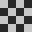
\includegraphics[width=4cm]{images/square.png}
\caption{A picture.}\label{fig:pic}
\end{figure}
Table~\ref{tab:counts} and Figure~\ref{fig:pic} on page~\pageref{fig:pic}; Theorem~\ref{thm:main}.
\subsection{More}
Vertical space between paragraphs and around headings can stretch and shrink a little, so that a page whose lines do not exactly fill it can still be set with its last line at the bottom. The amount of stretch is small, and most of it goes where a reader will not notice.

Notes at the foot of a page are collected separately from the main text. They take space from the page they appear on, and when there are too many some of them move to the next page, keeping their order and their numbers.

Figures and tables float. Instead of appearing exactly where they are mentioned they are placed at the top or bottom of a page, or on a page of their own, following preferences the author gives and limits the document class sets.
\end{document}
